\documentclass{article}\usepackage[]{graphicx}\usepackage[]{color}
% maxwidth is the original width if it is less than linewidth
% otherwise use linewidth (to make sure the graphics do not exceed the margin)
\makeatletter
\def\maxwidth{ %
  \ifdim\Gin@nat@width>\linewidth
    \linewidth
  \else
    \Gin@nat@width
  \fi
}
\makeatother

\definecolor{fgcolor}{rgb}{0.345, 0.345, 0.345}
\newcommand{\hlnum}[1]{\textcolor[rgb]{0.686,0.059,0.569}{#1}}%
\newcommand{\hlstr}[1]{\textcolor[rgb]{0.192,0.494,0.8}{#1}}%
\newcommand{\hlcom}[1]{\textcolor[rgb]{0.678,0.584,0.686}{\textit{#1}}}%
\newcommand{\hlopt}[1]{\textcolor[rgb]{0,0,0}{#1}}%
\newcommand{\hlstd}[1]{\textcolor[rgb]{0.345,0.345,0.345}{#1}}%
\newcommand{\hlkwa}[1]{\textcolor[rgb]{0.161,0.373,0.58}{\textbf{#1}}}%
\newcommand{\hlkwb}[1]{\textcolor[rgb]{0.69,0.353,0.396}{#1}}%
\newcommand{\hlkwc}[1]{\textcolor[rgb]{0.333,0.667,0.333}{#1}}%
\newcommand{\hlkwd}[1]{\textcolor[rgb]{0.737,0.353,0.396}{\textbf{#1}}}%
\let\hlipl\hlkwb

\usepackage{framed}
\makeatletter
\newenvironment{kframe}{%
 \def\at@end@of@kframe{}%
 \ifinner\ifhmode%
  \def\at@end@of@kframe{\end{minipage}}%
  \begin{minipage}{\columnwidth}%
 \fi\fi%
 \def\FrameCommand##1{\hskip\@totalleftmargin \hskip-\fboxsep
 \colorbox{shadecolor}{##1}\hskip-\fboxsep
     % There is no \\@totalrightmargin, so:
     \hskip-\linewidth \hskip-\@totalleftmargin \hskip\columnwidth}%
 \MakeFramed {\advance\hsize-\width
   \@totalleftmargin\z@ \linewidth\hsize
   \@setminipage}}%
 {\par\unskip\endMakeFramed%
 \at@end@of@kframe}
\makeatother

\definecolor{shadecolor}{rgb}{.97, .97, .97}
\definecolor{messagecolor}{rgb}{0, 0, 0}
\definecolor{warningcolor}{rgb}{1, 0, 1}
\definecolor{errorcolor}{rgb}{1, 0, 0}
\newenvironment{knitrout}{}{} % an empty environment to be redefined in TeX

\usepackage{alltt}

%%%%%%%%%%%%%%%%%%%%%%%%%%%%%%
%%% Preamble
%%%%%%%%%%%%%%%%%%%%%%%%%%%%%%

%%%
%%% Load packages
%%%

\usepackage{float}
\usepackage{mathtools}
\usepackage{geometry}
\geometry{legalpaper, margin=2in}
\usepackage{graphicx}


%%%
%%% Create new command to change color to blue
%%%

\newcommand{\blue}[1]{\textcolor{blue}{#1}}

%%%
%%% Set the graphics path to search for figures
%%%

\graphicspath{{../../Analysis/ResultsFigures/}}

%%%
%%% Title page
%%%

\title{Avian Species Richness in the United States}
\author{Your Name}
\date{Today's Date}

%%%%%%%%%%%%%%%%%%%%%%%%%%%%%%
%%% Begin document
%%%%%%%%%%%%%%%%%%%%%%%%%%%%%%
\IfFileExists{upquote.sty}{\usepackage{upquote}}{}
\begin{document}

%%%
%%% Set global R options
%%%



\maketitle

%%%
%%% Introduction
%%%

\section{Introduction}
We want to know whether avian species richness (the number of birds per state) is correlated with the size of the state, the average annual temperature, or the mean annual precipitation.

%%%
%%% Methods
%%%

\section{Methods}
To examine the relationship between avian species richness and the covariates area, temperature, and precipitation, we used the following multiple linear regression model:

%%
%% General Model Statement
%%

\begin{align}
y_i&=\beta_0+\beta_1x_{i,1}+\beta_2x_{i,2}+\beta_3x_{i,3}+\epsilon_i, \notag \\
\epsilon_i &\sim \text{Normal}(0,\sigma^2), \notag
\end{align}

where $y_i$ represents the number of species for the $i=1,\ldots,n$ state, $x_{i,1}$ represents the area of the  $i^{th}$ state, $x_{i,2}$ represents the mean annual temperature of the $i^{th}$ state, and $x_{i,3}$ represents the mean annual precipitation of the $i^{th}$ state. To estimate model parameters, we used \texttt{R} statistical software. The \texttt{R} script is shown, below.

%%%
%%% Analysis in R
%%%



%%%
%%% Results
%%%

\section{Results}
\subsection{Parameter Estimates}
The estimated intercept of our model, $\beta_0$, was 184. Thus, the expected number of species for a state with area equal to zero, temperature equal to zero, and precipitation equal to zero was 184. The estimated regression parameter for area, $\beta_1$,  was 0.0000385. Thus, as area increased by one km$^2$, the expected number of speciesincresed by 0.0000385. The estimated regression parameter for temperature, $\beta_2$,  was 4.10. As temperature increased by one degree Farenheit, the expected number of species incresed by 4.10. The estimated regression parameter for precipitation, $\beta_3$,  was -2.45. As temperature increased by one degree Farenheit, the expected number of species decresed by 2.45.  

%%
%% Fitted Model Statement
%%

Our fitted model is:
\begin{align}
y_i&=184+0.0000385x_{i,1}+410x_{i,2}-2.45x_{i,3}+\epsilon_i, \notag \\
\epsilon_i &\sim \text{Normal}(0,46^2), \notag
\end{align}

%%%
%%% Figures
%%%

\subsection{Figures}
To see the marginal relationship between $y_i$ and: $x_{i,1}$, $x_{i,2}$, and $x_{i,3}$, see Fig. 1


\begin{figure}
\begin{center}
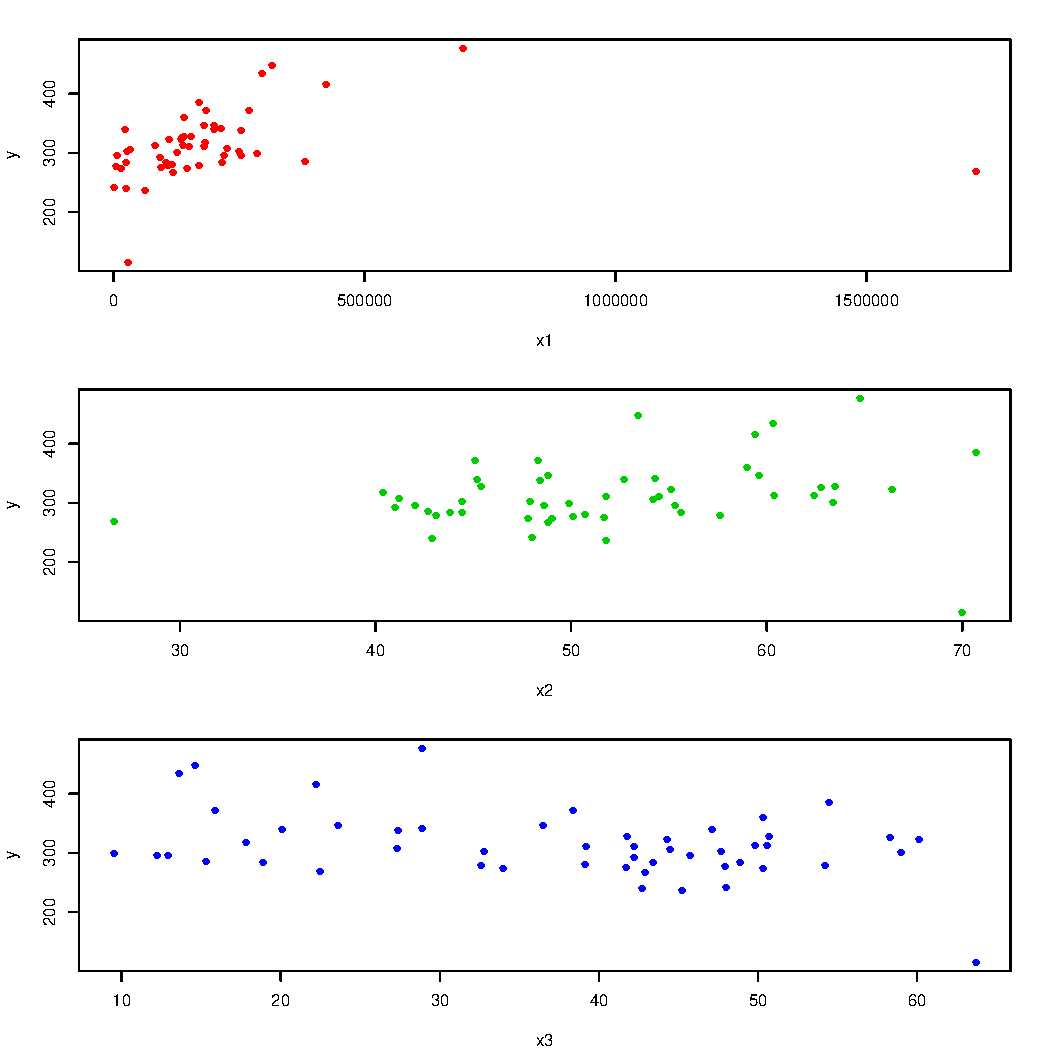
\includegraphics[width=10cm]{Figure1.pdf}
\caption{Marginal plot of the relationship between response variable and predictor variables.}
\end{center}
\end{figure}


%%%
%%% Tables
%%%

\subsection{Tables}
To see the parameter estimates and associated standard errors see Table 1.

\begin{table}[H]
\centering
\caption{Parameter estimates and SE of parameters from our fitted model.}
\begin{tabular}[t]{ c c c }
\hline
Parameter & Estimate & SE \\
\hline
 $\beta_0$ & 184 & 43.6 \\ 
 $\beta_1$ & 0.0000385 & 0.0000289 \\  
 $\beta_2$ & 410 & 0.889 \\
 $\beta_3$ & -2.45 & 0.552 \\
 $\sigma^2$ & 46 & - \\
 \hline
 \end{tabular}
\label{tab:estimates}
\end{table}

%%%
%%% Discussion
%%%

\section{Discussion}
After reconsidering, Alaska seems like an outlier. Re-fit the model by removing Alaska from the data (for an example of how to do this, see the commented code on line 34 of the "MainAnalysis.R" file. Update your manuscript accordingly.

\end{document}
